\documentclass[tikz,border=1pt,multi]{standalone}
\usetikzlibrary{shapes}
\begin{document}
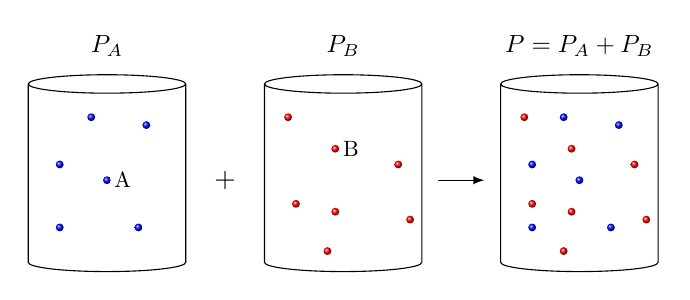
\begin{tikzpicture}[>=latex,shorten >=2pt,shorten <=2pt,shape aspect=1]

\node at (0,0) (A) [cylinder, shape border rotate=90, draw,minimum height=2.5cm,minimum width=2cm]
{};


    \shade [ball color=blue] (0,0) circle [radius=0.05cm];
    \shade [ball color=blue] (0.5,0.7) circle [radius=0.05cm];
    \shade [ball color=blue] (-0.2,0.8) circle [radius=0.05cm];
    \shade [ball color=blue] (0.4,-0.6) circle [radius=0.05cm];
    \shade [ball color=blue] (-0.6,-0.6) circle [radius=0.05cm];
    \shade [ball color=blue] (-0.6,0.2) circle [radius=0.05cm];
    
 \node[scale=0.8] at (0.2,0) {A};
 \node[scale=0.8] at (3.1,0.4) {B};
 
 \node[scale=0.9] at (0,1.7) {$P_{A}$};
 \node[scale=0.9] at (3,1.7) {$P_{B}$};
 \node[scale=0.9] at (6,1.7) {$P=P_A+P_{B}$};
 


\node at (3,0) (B) [cylinder, shape border rotate=90, draw,minimum height=2.5cm,minimum width=2cm]
{};

\shade [ball color=red] (2.9,0.4) circle [radius=0.05cm];
\shade [ball color=red] (3.7,0.2) circle [radius=0.05cm];
\shade [ball color=red] (2.4,-0.3) circle [radius=0.05cm];
\shade [ball color=red] (2.8,-0.9) circle [radius=0.05cm];
\shade [ball color=red] (2.9,-0.4) circle [radius=0.05cm];
\shade [ball color=red] (2.3,0.8) circle [radius=0.05cm];
\shade [ball color=red] (3.85,-0.5) circle [radius=0.05cm];


\node at (6,0) (C) [cylinder, shape border rotate=90, draw,minimum height=2.5cm,minimum width=2cm]
{};

\shade [ball color=blue] (6,0) circle [radius=0.05cm];
    \shade [ball color=blue] (6.5,0.7) circle [radius=0.05cm];
    \shade [ball color=blue] (5.8,0.8) circle [radius=0.05cm];
    \shade [ball color=blue] (6.4,-0.6) circle [radius=0.05cm];
    \shade [ball color=blue] (5.4,-0.6) circle [radius=0.05cm];
    \shade [ball color=blue] (5.4,0.2) circle [radius=0.05cm];

\shade [ball color=red] (5.9,0.4) circle [radius=0.05cm];
\shade [ball color=red] (6.7,0.2) circle [radius=0.05cm];
\shade [ball color=red] (5.4,-0.3) circle [radius=0.05cm];
\shade [ball color=red] (5.8,-0.9) circle [radius=0.05cm];
\shade [ball color=red] (5.9,-0.4) circle [radius=0.05cm];
\shade [ball color=red] (5.3,0.8) circle [radius=0.05cm];
\shade [ball color=red] (6.85,-0.5) circle [radius=0.05cm];

\node at (1.5,0)[] {$+$};

\draw[shorten >=0.2cm,shorten <=0.2cm,->] (B) -- (C);

\end{tikzpicture}
\end{document}